% !TEX root = ./Basilisk-Integrators20170724.tex


\begin{figure}[htb]
	\centerline{
	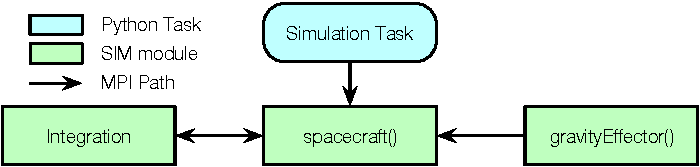
\includegraphics[]{Figures/integratorDiagram}
	}
	\caption{Illustration of the Integrator Diagram}
	\label{fig:intDiag}
\end{figure}


\section{Model Description}

\subsection{Overview}
The Basilisk integration capability is implemented in a modular manner such that different integrators can be assigned to the equations of motion that must be solved.  Figure~\ref{fig:intDiag} illustrates how the integrator functions relative to a dynamical systems model, here the {\tt SpacecraftPlus()} object.  The ODE's are provided by a sub-class of {\tt DynamicObject} which must be able to respond to the {\tt equationsOfMotion()} method.  How to integrated the state vector forward one time step is then handled by the {\tt integrate} method of the integrator class.  By default the {\tt DynamicObject} is integrated using a fixed time step 4th order Runge-Kutta method.  

Assume the dynamical system is given by
\begin{equation}
	\dot{\bm x} = \bm f(t, \bm x)
\end{equation}
The initial conditions are specified through $\bm x_{0} = \bm x(t_{0})$.  In integration time step is given through $h$.  

\subsection{Implemented Integrators}

\subsubsection{4th Order Runge Kutta - Default Integrator}
A standard fixed time step 4th order Runge Kutta integrator is enabled by default.  The 4 $k_{i}$ values are defined as
\begin{align}
	\bm k_{1} &= \bm f(t_{n}, \bm x_{n}) \\
	\bm k_{2} &= \bm f(t_{n} + \frac{h}{2}, \bm x_{n} + \frac{h}{2} \bm k_{1}) \\
	\bm k_{3} &= \bm f(t_{n} + \frac{h}{2}, \bm x_{n} + \frac{h}{2} \bm k_{2}) \\
	\bm k_{4} &= \bm f(t_{n} + h, \bm x_{n} + h \bm k_{3}) 
\end{align}
The states at the next integration time $t_{n+1} = t_{n} + h$ is
\begin{equation}
	\bm x_{n+1} = \bm x_{n} + \frac{h}{6} \left(
		\bm k_{1} + 2 \bm k_{2} + 2 \bm k_{3} + \bm k_{4}
	\right)
\end{equation}


\subsubsection{2nd Order Runge Kutta (Heun's Method)}
A 2nd order Runge-Kutta method is implemented through Heun's method.\footnote{\url{http://goo.gl/SWdyBZ}} The 2 $k_{i}$ values are defined as
\begin{align}
	\bm k_{1} &= \bm f(t_{n}, \bm x_{n}) \\
	\bm k_{2} &= \bm f(t_{n} + h, \bm x_{n} + h \bm k_{1}) 
\end{align}
The states at the next integration time $t_{n+1} = t_{n} + h$ is
\begin{equation}
	\bm x_{n+1} = \bm x_{n} + \frac{h}{2} \left(
		\bm k_{1} +  \bm k_{2}
	\right)
\end{equation}


\subsubsection{1st Order Runge Kutta (Euler's Method)}
A first order Runge-Kutta method is implemented through Euler's method. The one $k_{1}$ value is defined as
\begin{align}
	\bm k_{1} &= \bm f(t_{n}, \bm x_{n}) 
\end{align}
The states at the next integration time $t_{n+1} = t_{n} + h$ is
\begin{equation}
	\bm x_{n+1} = \bm x_{n} + h
		\bm k_{1}
\end{equation}
